\documentclass[sigconf,nonacm]{acmart}
\usepackage{booktabs}
\graphicspath{{../figures/}}

\begin{document}

\title{Authorship Needs Provenance, Not Prediction}

\author{Anonymous Author(s)}
\affiliation{%
  \institution{Position paper, draft 1}
  \city{}
  \country{}
}

\begin{abstract}
AI writing detectors such as Pangram and Turnitin are increasingly used to adjudicate \emph{authorship}---who or what wrote a text---in publishing, education, and journalism. Detectors promise to settle this question by predicting the text's origin from its style. We call the mismatch between what detectors can measure and what authorship disputes need the \textbf{provenance-text gap}: authorship is a property of the writing \emph{process}, while detection observes only the \emph{product}. The belief that a sufficiently accurate classifier can close this gap---the \textbf{detectability fallacy}---is contradicted by four measurements we report here. (1) In arXiv abstracts and Hacker News comments, the lexical ``tells'' associated with AI rise after ChatGPT's release and then collapse below baseline as writers learn to avoid them, while structural patterns persist: the detector's target moves because the detector exists. (2) Across eight corpora, no marker separates AI text from all human registers; several ``AI tells'' are more prevalent in human writing, and both of our 2023-era AI corpora are barely marked by the tell vocabulary at all. (3) Transparent classifiers trained on matched human/AI pairs reach 0.98+ AUC in-domain but collapse to 0.56--0.81 across AI corpora, and their false-positive rates at fixed thresholds range from 0\% to 73\% depending on the human corpus---error concentrates by register and by author. (4) At the scale and accuracy vendors themselves claim, deployed detection yields tens to hundreds of false accusations per day, and for writers in high-error registers a flag shifts the probability of AI authorship by barely more than a coin flip. We argue that authorship disputes need \textbf{provenance}---evidence about the writing process: drafts, version histories, disclosure contracts, attestations, and audit trails---with detection demoted to triage. The next generation of authorship tools should not be better scores; it should be better evidence.
\end{abstract}

\keywords{AI text detection, authorship attribution, false positives, stylometry, provenance, writing process, academic integrity}

\maketitle

\section{Introduction}

The fastest way to adjudicate a dispute about who wrote a text is to run it through a detector. In practice, this often means submitting a manuscript to a service such as Pangram, an essay to Turnitin, or a news article to one of a dozen free tools, and receiving a score: 78.3\% AI, in the case that has become the publishing industry's reference point. When Hachette Book Group withdrew Mia Ballard's novel \emph{Shy Girl} after such a score, it set the precedent that a stylometric prediction can end a writing career~\cite{r1}. Authors have lost book deals, students have failed courses, and job applicants have been rejected on the strength of these numbers.

By \emph{detection}, we mean any method that infers a text's generative origin from properties of the finished text alone. By \emph{provenance}, we mean evidence about the process that produced it: drafts, edit histories, disclosure statements, attestations by people or institutions, and records that can be inspected and contested. The distinction matters because the thing being disputed---authorship---is a fact about process, not product. Two texts can be stylistically identical and have different authors; the same author can produce texts in different registers.

This article makes one claim: \textbf{authorship disputes need provenance, not prediction.} Detectors classify products; authorship is a process property. No improvement in classifier accuracy changes this category error, which we call the \emph{provenance-text gap} and elaborate in Section~2 as the \emph{detectability fallacy}.

The novelty is not the observation that detectors are inaccurate. Independent evaluations have found commercial tools unreliable~\cite{r4}, biased against non-native English writers~\cite{r3}, and breakable by paraphrase~\cite{r5,r17}, with theoretical results bounding how well any detector can perform as AI text approaches human text in distribution~\cite{r5}. Detection has also accrued genuine methodology---statistical forensics designed to let non-experts inspect token probabilities~\cite{r11}, experiments measuring what human readers can detect~\cite{r12}, zero-shot likelihood criteria~\cite{r13}, and feature-based classifiers that generalize across domains~\cite{r14}, with surveys mapping the threat landscape~\cite{r15}. Our contribution is to connect three threads that this literature treats separately. First, we show with our own measurements that detection is not merely inaccurate but \emph{reflexive}: it reshapes the writing it surveys, moving its own target (Section~3.2). Second, we show that error is not merely present but \emph{concentrated}, by register and by author, in ways that population-level accuracy statistics conceal (Sections~3.3--3.5). Third, we argue that the correct response is architectural, not incremental: process evidence, structured and standardized, as the substrate of authorship adjudication (Section~4).

All measurements in Section~3 are ours, collected and computed for this article from public corpora: 64,824 Hacker News comments (2015--2026), 5{,}880 arXiv cs.CL abstracts (2010--2026), 6{,}000 matched pairs of human Wikipedia introductions and GPT-3.5 completions, 3{,}236 matched pairs of human and ChatGPT answers from HC3, and 11{,}066 segments from 41 title-verified works of pre-LLM literature. Every number we report can be recomputed from the scripts and data sources described in Section~3.1.

\section{The Detectability Fallacy}

A detector promises to classify a text. An authorship proceeding needs to classify a \emph{history}: a sequence of decisions, revisions, and tool uses by a specific person, spread over time. The belief that a sufficiently accurate classifier can substitute for that history is the detectability fallacy. It is understandable: classifiers report confident numbers, institutions need answers at scale, and the alternative---asking for evidence about how something was written---sounds quaint. But four commitments that authorship adjudication requires are structurally absent from prediction over finished text.

\noindent\textbf{Product without process.} The detector sees a document; the dispute is about how it came to exist. Pangram itself distinguishes ``AI-generated'' from ``AI-assisted'' text via what it calls autonomous authorship decisions---if a writer supplies bullet points for ChatGPT to expand, that counts as generated~\cite{r1}---but no score over the finished text can observe that distinction; it can only guess at it. The same is true of the boundaries institutions actually argue about, from Nobel laureate Olga Tokarczuk's collegial use of drafting dialogue to novelist Andrea Bartz's refusal of any generative assistance at all~\cite{r1}. These are facts about process that prediction over product cannot recover.

\noindent\textbf{Average error without individual error.} A false-positive rate is a population statistic; an accusation lands on one writer. Pangram's chief executive claims a 1-in-10,000 false-positive rate for the company's latest model, while conceding it is ``definitely not zero, especially when we're scanning millions of documents a day''~\cite{r1}. Both halves of that sentence are true, and their conjunction is the problem: a population-average error rate says nothing about the rate for the \emph{accused} writer's register, background, or neurotype. A detector can be 99.99\% accurate on average and nearly a coin flip for exactly the person it flags, as we quantify in Section~3.5. Detection studies have documented the concentration: more than half of essays by non-native English speakers were classified as AI-generated by widely used detectors, a 61.3\% average false-positive rate, while native essays passed almost universally~\cite{r3}.

\noindent\textbf{Measurement without immunity to the measurement.} Detectors change what they measure. Writers and their editors now avoid words, punctuation, and constructions associated with AI output~\cite{r1}; the association itself is learned from public discourse about detectors. A tool that flags ``delve'' teaches writers to shun ``delve,'' after which the tool's signature is stale and the writers' prose is distorted. Yakura et al.\ documented the rise of ChatGPT-preferred words in spontaneous human speech after the chatbot's release---and their fall below baseline once ``delve'' became stigmatized~\cite{r2}. We replicate this spike-and-purge pattern in written academic prose and add a finding they do not report: the \emph{structural} markers of AI style persist through the lexical purge (Section~3.2). Detectors do not merely fail at their task; they distort the population they survey, which is a property no accuracy improvement fixes, because the improvement itself accelerates the distortion.

\noindent\textbf{Verdicts without audit trails.} A detector emits a number, not an argument. Weber-Wulff et al.'s evaluation of fourteen tools concluded that ``a student accused of unauthorised content generation only on this basis would have no possibility for a defence''~\cite{r4}. Even a \emph{correct} score is unauditable in the way an accusation requires: it cannot show which passages drove the verdict, what evidence would rebut it, or how confident the system was for writers like this one. The result is what we call \textbf{accusation debt}: a growing liability of verdicts resting on unexplained scores, scattered across publishers' workflows, universities' dashboards, and editors' inboxes, each individually deniable and collectively unrevisable.

The four deficits compound. Because verdicts are unexplained, error concentration stays invisible; because error stays invisible, adaptation pressure keeps rising; because writers adapt, signatures decay; and because signatures decay, vendors retrain, restarting the cycle. None of this is a calibration bug. It is what prediction looks like when applied to a process question under adversarial pressure.

\section{Evidence}

We report four probes: a time series of markers in human-written venues (Section~3.2), a cross-register comparison of human and AI marker rates (Section~3.3), a family of transparent classifiers that we train and then break in controlled ways (Section~3.4), and the arithmetic of accusation at claimed accuracy and scale (Section~3.5). Together they ground the fallacy's four deficits with numbers.

\subsection{Corpora and markers}

We measure the stylistic markers that public discourse treats as ``AI tells'': the em-dash; a 32-item \emph{slop lexicon} of words associated with chatbot prose (delve, tapestry, testament, pivotal, myriad, robust, seamless, and kin); the rule-of-three (triadic lists); the ``not X, but Y'' construction; ``not only \ldots\ but also''; connectives such as \emph{moreover}; and sentence- and word-level statistics (mean and standard deviation of sentence length, type-token ratio, mean word length). Feature extraction is count-based and fully specified in our scripts; rates are pooled per corpus with 95\% Poisson intervals.

Table~\ref{tab:corpora} summarizes the corpora. Two design choices matter. First, both AI corpora are from 2023 models (GPT-3.5 completions in a Wikipedia register; ChatGPT 3.5-turbo in a Q\&A register), matched topic-for-topic to human counterparts written before ChatGPT. Second, all ``human'' labels after 2022 are unverifiable in principle---an increasing share of public writing is AI-assisted---so our time series should be read as measuring the \emph{ecosystem}, not individuals. This labeling crisis is not incidental; it is part of our argument, and we return to it in Section~7.

\begin{table}[t]
\centering
\small
\caption{Corpora.}
\label{tab:corpora}
\begin{tabular}{@{}lrrl@{}}
\toprule
Corpus & Docs & Words & Period / nature \\
\midrule
Hacker News comments & 64{,}824 & 5.80M & 2015--2026, monthly \\
arXiv cs.CL abstracts & 5{,}880 & 0.90M & 2010--2026, quarterly \\
GPT-wiki-intro (AI) & 6{,}000 & 0.80M & GPT-3.5, wiki register \\
Wikipedia intros (human) & 6{,}000 & 1.13M & Same topics, 2022 \\
HC3 ChatGPT answers (AI) & 3{,}236 & 0.63M & GPT-3.5-turbo, Q\&A \\
HC3 human answers & 3{,}236 & 0.53M & Pre-ChatGPT Q\&A \\
Project Gutenberg & 11{,}066 & 6.76M & 41 pre-LLM books, 23 authors \\
\bottomrule
\end{tabular}
\end{table}

\subsection{The adaptation curve: tells rise, then are purged; structures persist}

If detectors and the discourse around them shape writing, marker frequencies in human-written venues should break around ChatGPT's release (November 2022) and again around the public naming of specific tells. They do.

In arXiv cs.CL abstracts, the ``delve'' family sits at zero to 3 per 100K words from 2010 through 2023 (four occurrences in fourteen years of sampled abstracts), spikes to 13.3 per 100K in 2024 (nine occurrences in 67{,}800 words), then collapses: one occurrence in 2025, zero in 2026 (upper 95\% bound 4.1 per 100K). The slop lexicon tells the same story at lower frequency resolution: 91 per 100K words in 2020, 136 in 2022, 253 in 2025, then a 45\% drop in 2026. This is the spike-then-purge pattern that Yakura et al.\ documented in speech~\cite{r2}, reproduced here in \emph{written academic prose} (Figure~\ref{fig:adaptation}), and it is difficult to explain by contamination alone: AI assistance in writing kept growing through 2025--2026, while the named lexical tells collapsed. The purge is behavior, not usage.

The striking exception is structure. Triadic lists---the rule-of-three---average 0.65 per 1K words in 2010--2019 and 1.97 per 1K in 2023--2026, a 3.0$\times$ elevation that persists through the 2026 lexical purge. Writers (or their tools) have abandoned the \emph{words on the folk list} but kept the \emph{patterns not on it}. Avoidance tracks the list, not the underlying distribution: humans are not avoiding AI-likeness; they are avoiding the folk theory of AI-likeness.

Hacker News shows the complementary regime. The slop lexicon, flat at 12--17 per 1K words for a decade, rises 73\% in 2026 relative to the 2015 baseline---the register is absorbing AI-associated vocabulary rather than purging it. Em-dashes, ``moreover,'' and ``delve'' stay near the floor throughout. The same ecosystem, sampled at different detector-salience, moves in opposite directions: the high-stakes academic register purges tells; the forum register hybridizes. Both movements are consistent with detector pressure---the one mechanism for style change around AI text that has been directly documented~\cite{r2}---and neither is stable. A detector trained on either snapshot is trained on a moving target that its own deployment may be moving.

\begin{figure*}[t]
\centering
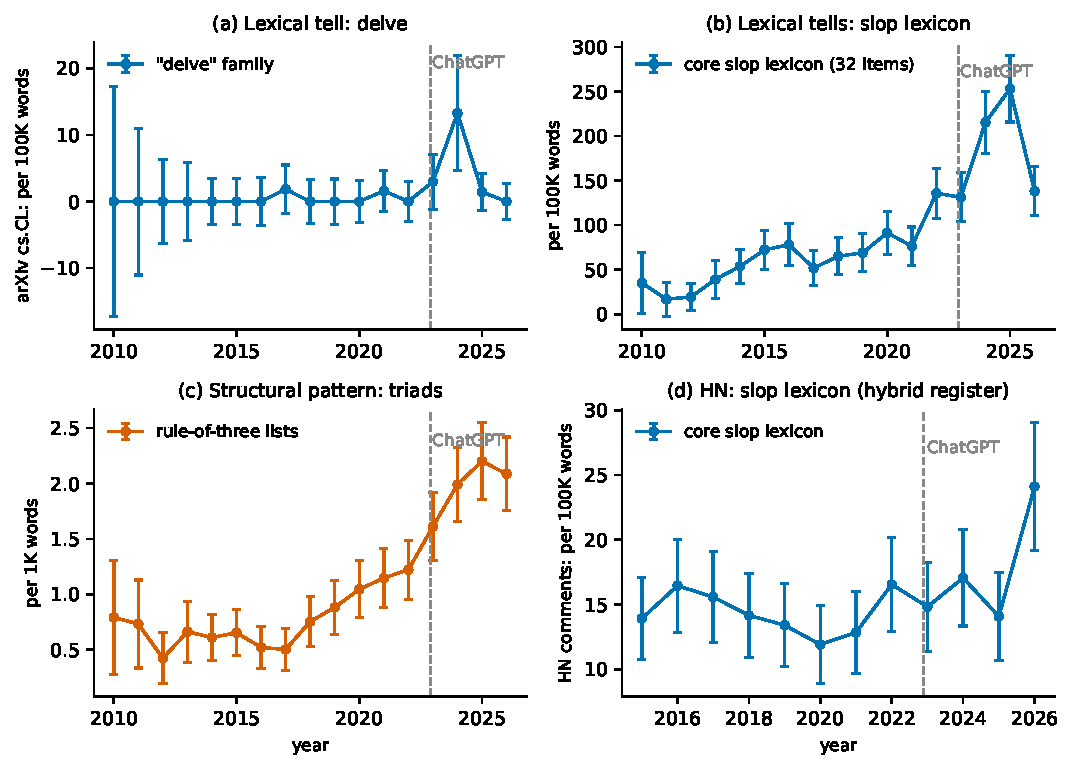
\includegraphics[width=0.98\textwidth]{e1_adaptation.pdf}
\caption{The adaptation curve. \emph{Top-left:} ``delve''-family rate per 100K words in arXiv cs.CL abstracts with 95\% Poisson intervals; the 2026 zero-rate upper bound is 4.1. \emph{Top-right:} core slop-lexicon rate, same corpus. \emph{Bottom-left:} rule-of-three rate per 1K words, which persists through the lexical purge. \emph{Bottom-right:} slop-lexicon rate in Hacker News comments, flat for a decade, rising 73\% in 2026 (Section~3.2).}
\Description{Four line charts with 95\% Poisson intervals showing lexical marker rates over time in arXiv abstracts and Hacker News comments: delve-family and slop-lexicon rates spike after 2023 and collapse in 2026 in arXiv, rule-of-three rates persist, and Hacker News slop rates rise 73 percent in 2026.}
\label{fig:adaptation}
\end{figure*}

\subsection{The moving target: no marker separates AI from all human registers}

The folk theory holds that certain markers indicate AI. Across our eight corpora (Figure~\ref{fig:overlap}), no marker on the folk list does so, and several invert.

\begin{itemize}
\item \textbf{Em-dashes.} Human pre-LLM literature uses 5.7 per 1K words; human Wikipedia intros 3.1; the GPT-3.5 completion corpus 2.5; ChatGPT Q\&A answers 0.03. On this marker, the \emph{humans} are the outliers in the folklore's direction: the AI corpora use fewer em-dashes than their matched human counterparts. (Reports on 2025--2026 models point the other way~\cite{r1}; the sign of the tell is not even stable across model generations.)
\item \textbf{``Not X, but Y.''} A construction now treated as an AI fingerprint---and one for which a Nigerian author lost a \$2M deal, since ``not X, but Y'' is idiomatic in Yoruba-influenced English~\cite{r1}---is in our corpora a \emph{human} marker: 3.5--3.8 per 10K words in Victorian literature and pre-LLM forum writing, 0.9--1.4 in matched human Q\&A and Wikipedia text, versus 0.3--0.8 in the two AI corpora. Penalizing it penalizes humans, and especially humans from rhetorical traditions that use it.
\item \textbf{The slop lexicon.} Neither 2023 AI corpus is meaningfully slop-marked: 0.09--0.11 per 1K words, the same as their human counterparts (0.10--0.11) and below pre-LLM forum writing (0.15). ``Delve'' is nearly absent from both (0.0--0.16 per 100K). The tell vocabulary that writers are purging from their prose was never strongly present in this generation of AI output; it characterizes the \emph{post-2023 hybrid ecosystem} (arXiv 2023--2026: 1.84 per 1K; delve 4.3 per 100K), where human and machine writing have already mixed.
\item \textbf{Rule-of-three.} The one marker consistently elevated in both AI corpora relative to matched humans (1.66 vs.\ 1.06; 2.32 vs.\ 0.89 per 1K words) and in post-2023 academic prose (1.98 vs.\ 0.65). It is also, per Section~3.2, the marker that survives the human purge. The signal that actually tracks AI style is the one nobody is avoiding---because it is not on the list.
\end{itemize}

\begin{figure}[t]
\centering
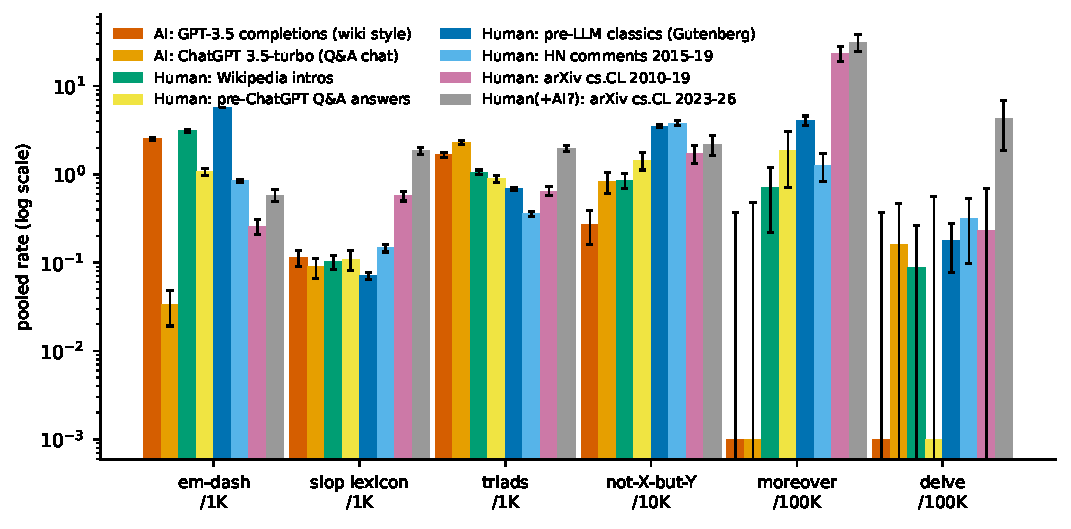
\includegraphics[width=\linewidth]{e2_overlap.pdf}
\caption{Marker rates per corpus (log scale): em-dash and ``not X, but Y'' per 1K/10K words respectively, rule-of-three and slop lexicon per 1K words, across human (blue) and AI (red) corpora spanning registers. No marker separates AI text from all human registers; several invert (Section~3.3).}
\Description{Grouped bar chart on a log scale showing marker rates for eight corpora; AI and human bars overlap for every marker, and for em-dashes and not-X-but-Y the human bars exceed the AI bars.}
\label{fig:overlap}
\end{figure}

The pattern across markers is not that AI and human writing are inseparable; it is that \emph{which} features separate them depends on model generation, register, and year. This is register variation in the classical sense---linguistic features that co-vary systematically with communicative situation, not with writer identity~\cite{r16}. A detector is a snapshot of a particular human/AI pair at a moment in time, presented as a general truth about machines and people.

\subsection{Anatomy of a detector: seductive in-domain, brittle across pairs, punishing by register}

To make the snapshot claim concrete, we trained three transparent classifier families on each of two matched human/AI pairs: logistic regression on the nine folk markers (``folk''), TF-IDF word uni/bigrams with logistic regression (``tfidf''), and TF-IDF character 3--5-grams (``char''---the feature family classical authorship attribution actually uses). W = Wikipedia-intro pair; H = chat Q\&A pair. We then evaluated each model the way vendors do not: on the \emph{other} AI corpus, and on human corpora from other registers.

Table~\ref{tab:grid} reports the grid. Three results deserve emphasis.

\begin{table*}[t]
\centering
\small
\caption{Classifier performance. AUC on held-out in-domain data; transfer = AUC on the other pair; FPR at the threshold achieving 95\% true-positive rate in-domain, evaluated on pre-LLM human corpora (Gutenberg literature, HN 2015--2019, arXiv 2010--2019) and post-2023 arXiv.}
\label{tab:grid}
\begin{tabular}{@{}llrrrrrrr@{}}
\toprule
Pair & Model & In-domain AUC & Transfer AUC & In-domain FPR@95 & Gutenberg FPR & HN-pre FPR & arXiv-pre FPR & arXiv-post FPR \\
\midrule
W & folk & 0.834 & 0.560 & 0.58 & 0.40 & 0.73 & 0.56 & 0.48 \\
W & tfidf & 0.981 & 0.811 & 0.09 & 0.00 & 0.27 & 0.16 & 0.06 \\
W & char & 0.976 & 0.723 & 0.14 & 0.00 & 0.65 & 0.19 & 0.04 \\
H & folk & 0.921 & 0.620 & 0.29 & 0.26 & 0.06 & 0.47 & 0.40 \\
H & tfidf & 0.995 & 0.721 & 0.03 & 0.00 & 0.00 & 0.05 & 0.04 \\
H & char & 0.993 & 0.671 & 0.04 & 0.00 & 0.01 & 0.09 & 0.10 \\
\bottomrule
\end{tabular}
\end{table*}

\noindent\emph{In-domain accuracy is real and seductive.} The tfidf and char models reach 0.98--0.995 AUC on their own pairs, with in-domain false-positive rates of 3--14\% at a 95\% detection threshold---vendor-grade numbers. We do not doubt that Pangram's in-lab evaluations are as good as claimed. OpenAI's own classifier, retired five months after launch for a ``low rate of accuracy''~\cite{r9}, shows how quickly such claims meet their shelf life.

\noindent\emph{The signature does not transfer.} The same models, asked to distinguish the \emph{other} pair of human and AI text, fall to 0.56--0.81 AUC. The folk model trained on W is nearly at chance (0.56) on H. What a detector learns is not ``AI style'' but ``this model, this register, this year''---which is why retraining is continuous and why a score calibrated last quarter is a guess this quarter.

\noindent\emph{Error concentrates by register---and by author.} At W-calibrated thresholds, the folk model flags 73\% of pre-LLM Hacker News comments and 56\% of pre-LLM arXiv abstracts; the char model, the authorship-attribution workhorse, flags 65\% of the same comments. Even the H-pair tfidf model---the best cross-register case in our grid---still flags 5\% of 2010--2019 arXiv abstracts, above its own 3.4\% in-domain error. Within the Gutenberg corpus the concentration is stark (Figure~\ref{fig:fpr}): the W folk model flags 99\% of segments from D.~H. Lawrence's \emph{Sons and Lovers}, 79\% of Wilde, 77\% of London, and 73\% of Doyle, against 13\% of Melville and 15\% of Thackeray. Being flaggable is a stable property of \emph{who you are} as a stylist, not of what you did.

Finally, the interpretability results undermine the folk theory from the machine's side. The tfidf model's most AI-indicative terms are not \emph{delve}, \emph{tapestry}, or any item of the folk list; they are register boilerplate---``born in,'' ``died,'' ``was founded,'' ``including,'' ``it is important''---while its most human-indicative terms are informal markers (``but,'' ``my,'' ``you,'' ``hi,'' ``like''). The discriminative vocabulary is topic and register, not origin. And in the folk model's weights, the em-dash coefficient is \emph{negative} in both pairs (AI uses fewer), as is type-token ratio: the two most-cited folk tells either point the wrong way or measure register diversity. Writers purging the folk list are not fooling these classifiers; they are, at best, fooling the folklore.

\begin{figure}[t]
\centering
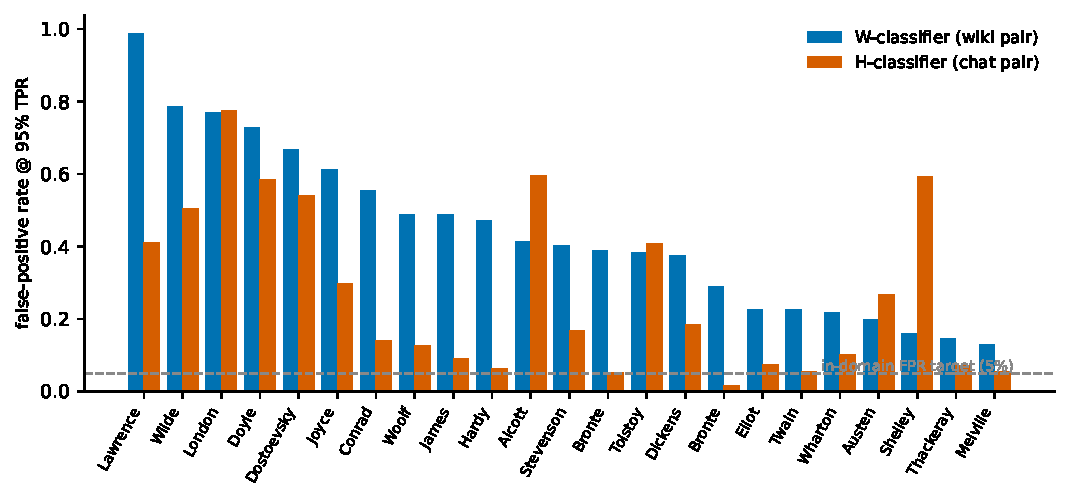
\includegraphics[width=\linewidth]{e3_fpr_by_author.pdf}
\caption{False-positive rate at the W folk model's 95\%-TPR threshold, by Gutenberg author. Spread: 13\% (Melville) to 99\% (Lawrence), within a single register of pre-LLM literature (Section~3.4).}
\Description{Bar chart of per-author false-positive rates for 23 Victorian-era authors, ranging from 13 percent for Melville to 99 percent for Lawrence.}
\label{fig:fpr}
\end{figure}

\subsection{The arithmetic of accusation}

Individual numbers above are measurements; the accusation pipeline is arithmetic, and it does not need our corpora to be damning.

\paragraph*{\emph{Scale.}} At the vendor-claimed 1-in-10,000 false-positive rate, scanning 5 million documents per day of which 20\% are human-written yields 100 false accusations per day---25{,}000 per year at 250 working days. Even at 90\% AI prevalence, it is 50 per day. The chief executive's concession that the rate is ``not zero'' at scale is, in expectation, a standing monthly news story about a destroyed writer.

\paragraph*{\emph{The base-rate inversion for outlier writers.}} For a writer whose personal false-positive rate equals the population average (1 in 10,000), a flag at a 95\%-sensitivity operating point shifts the probability of AI authorship from 20\% prior to 99.96\%---a genuinely damning event. But Section~3.4 measured per-register false-positive rates of 16--73\% for exactly the styles such systems will meet. For a writer with a 30\% personal FPR, the same flag yields a posterior of 44\%; at 56\%, it yields 30\%---\emph{below the ``more likely than not'' bar that misconduct findings require}. The same score, with the same calibration, is near-conclusive for one writer and nearly uninformative for another, and nothing in the delivered score distinguishes the two.

\paragraph*{\emph{Evidence per flag.}} For an accused writer, the evidentiary value of a flag is the likelihood ratio TPR/FPR. Under the W folk model, that ratio ranges from 1.0 (Lawrence: a flag is as likely if human) to 7 (Melville) across our 23 authors (Figure~\ref{fig:lr})---every value below the 19 that legal evidence standards treat as ``strong,'' and for several authors below even the ``weak'' band. A regime in which the strongest commonly-admitted evidence against a writer is, for that writer, statistically consistent with innocence is not an accuracy problem; it is an evidentiary category error.

\begin{figure}[t]
\centering
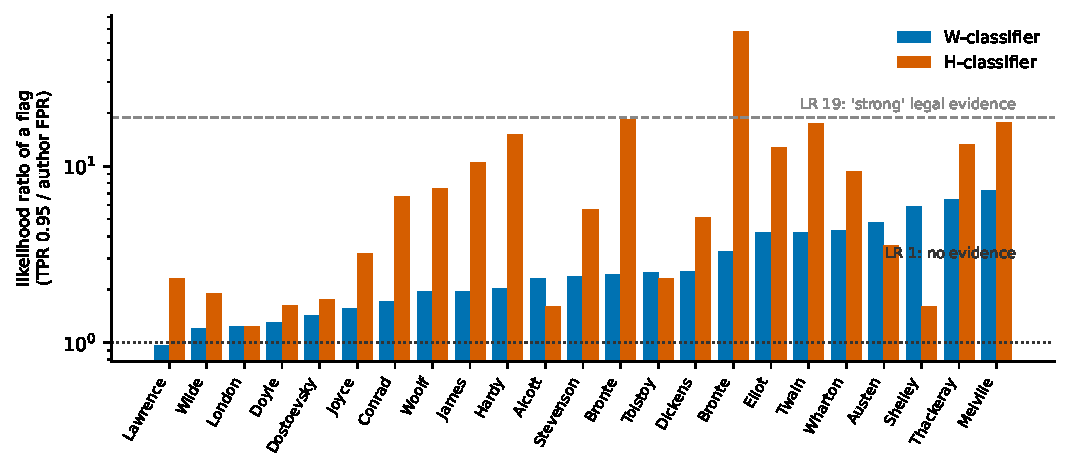
\includegraphics[width=\linewidth]{e4_lr_by_author.pdf}
\caption{Likelihood ratio TPR/FPR of a flag under the W folk model, by Gutenberg author. Every author's ratio lies below the ``strong evidence'' threshold of 19; for the low end, a flag carries essentially no information (Section~3.5).}
\Description{Bar chart of per-author likelihood ratios under the W folk model, all values between 1.0 and 7.3, below the legal strong-evidence threshold of 19.}
\label{fig:lr}
\end{figure}

\section{What Provenance Adds}

Prediction over the finished text cannot bear the weight of an accusation. What would? Authorship disputes need evidence about process, and process evidence can be structured. We propose that the unit of adjudication shift from the \emph{score} to the \textbf{provenance record}: a machine-readable, writer-controlled account of how a text came to exist. Provenance does not replace detection; it replaces \emph{detection as evidence}. Five surfaces define it.

\noindent\textbf{Process record.} Drafts, edit histories, and timestamps that document a text's development. Version history already exists in every word processor and repository; the missing piece is a standard for \emph{presenting} it, selectively and verifiably, to an adjudicator. A writer who can show six weeks of revision is making a claim a classifier cannot touch; a writer who cannot---because they write in one pass, or on paper---must not be penalized for it (Section~6).

\noindent\textbf{Disclosure contracts.} Structured declarations of AI assistance at graded levels, from ``none'' through ``mechanical assistance'' (grammar, spelling, rephrasing) to ``co-drafting'' and ``generation from outline.'' Pangram's own generated/assisted distinction~\cite{r1} is an implicit disclosure taxonomy; the publishing industry lacks a shared one, which is why the same practice reads as fraud in one house and diligence in another. Disclosure contracts make the norm explicit and the dispute bounded: the question shifts from ``is there AI in this text?''---unanswerable---to ``does the disclosed process match the contract?''---answerable.

\noindent\textbf{Attestation.} Signed statements binding the process record to accountable parties: the writer, an editor, an institution, a classroom proctor. Content-provenance infrastructure such as C2PA already defines signed manifests and ingredient lists for media~\cite{r10}; text authorship needs the same plumbing. Attestation is what converts ``the file says so'' into ``someone vouches, with consequences.''

\noindent\textbf{Audit and due process.} Contested verdicts must expose their basis: which passages drove the decision, what the model's error rate is \emph{for writers like the accused}, and what evidence would rebut the finding. This is the trace obligation that detection verdicts currently lack~\cite{r4}, and it is not optional at accusation stakes---the strongest research prototype in the field explicitly warns against automated punitive use~\cite{r14}. Regulatory analogues exist in credit scoring and adverse-action notices; authorship tools are overdue for the same treatment.

\noindent\textbf{Preservation of style outliers.} Because error concentrates (Sections~3.3--3.5), any adjudication regime must actively protect the registers and traditions that prediction penalizes: non-native rhetorical patterns such as Yoruba-influenced ``not X, but Y''~\cite{r1,r3}, formulaic academic prose, neurodivergent writing styles, and the plain styles of low-stakes forums. A provenance regime does this structurally---process evidence does not care how you write---whereas no threshold calibration can do it, because the concentration is in the features, not the threshold.

Provenance, like protocol interfaces in agent engineering, is a synthesis layer rather than an invention: version control, disclosure norms, signed manifests, and due process all exist. What does not exist is their composition at the boundary where an accusation is made.

\section{Positioning}

Our argument sits at the junction of four literatures, and borrows from each without being any of them.

\emph{Detection reliability research} has documented the failure modes we quantify: accuracy below vendor claims across fourteen tools~\cite{r4}; 61.3\% false positives on non-native essays~\cite{r3}; collapse under recursive paraphrasing, with a theoretical bound tying detector AUROC to the total-variation distance between human and AI text distributions---a bound that tightens toward chance as models improve~\cite{r5}. Empirical attack studies agree with the theory: an 11B-parameter paraphraser drops a leading zero-shot detector from 70.3\% to 4.6\% accuracy at constant false-positive rate~\cite{r17}, and detectors trained against adaptive attackers still face a moving frontier~\cite{r18}. We extend this line from \emph{accuracy} to \emph{evidentiary adequacy}: even a detector that met its accuracy claims would still fail the four commitments of Section~2, because the failures are structural, not statistical.

\emph{Watermarking} moves provenance to generation time, embedding signals in model output~\cite{r6}. It is the strongest pro-detection proposal---but it certifies only cooperating models, degrades with length and paraphrase~\cite{r5}, and cannot speak to human writing at all. It complements, not replaces, writer-side provenance.

\emph{Content provenance standards} (C2PA and related~\cite{r10}) provide the cryptographic and schema substrate for attestation; they were designed for images and media, and their extension to the \emph{process} of writing---drafts, not pixels---is an open engineering problem we flag in Section~7.

\emph{Education-integrity practice} has already moved toward process: oral defenses, in-class writing, and portfolio assessment, with multiple independent evaluations concluding that detection scores should not be used as evidence of misconduct~\cite{r3,r4}. Systematic reviews of AI in higher education conclude the same thing from the institutional side: adoption is running well ahead of evidence~\cite{r19}. Our proposal generalizes that instinct to publishing and journalism, and gives it a technical shape.

Two further strands anchor our empirical choices. Yakura et al.'s finding that ChatGPT's lexical preferences propagate into spontaneous speech---and recede once stigmatized~\cite{r2}---is the cleanest prior evidence of detector-adjacent reflexivity; our Section~3.2 replicates its shape in written academic prose and extends it to structure. And the matched-corpus design we use for Section~3.4 follows the human/AI comparison tradition of HC3~\cite{r7} and GPT-wiki-intro~\cite{r8}, with the twist that we treat the two AI corpora as \emph{different points in AI style space}, which is precisely what the transfer collapse demonstrates.

\section{Principles and Tradeoffs}

Five principles govern a provenance regime worth building.

\begin{enumerate}
\item \textbf{Process over product.} The evidentiary unit is the history, not the artifact. Scores may triage; histories adjudicate.
\item \textbf{Graduated disclosure.} Assistance is a spectrum~\cite{r1}; disclosure contracts must grade it, and institutions must set norms per context. Binary ``AI or not'' regimes recreate the category error inside the disclosure form.
\item \textbf{Writer-controlled, local-first.} A process record that institutions harvest by default is surveillance. Draft histories should live with the writer and be \emph{presentable} on demand---selectively, verifiably, and without bulk exfiltration. The privacy failure mode of provenance is the panopticon; the design answer is local-first attestation, the way password managers prove possession without revealing secrets.
\item \textbf{Error honesty.} Any deployed detector should be obligated to publish error rates \emph{by subpopulation and register}, updated as the population drifts---the concentration curves of Section~3.4, not a single number. Where a vendor cannot measure subpopulation error, it cannot claim the score means anything for that population.
\item \textbf{Proportionate burden.} Not every text needs provenance. Spam filtering, content moderation triage, and low-stakes screening are legitimate prediction uses. Provenance is for accusation stakes: publication withdrawal, misconduct findings, contract termination, grade penalties.
\end{enumerate}

The costs are real and we do not minimize them. Provenance infrastructure is engineering work---schemas, tools, workflow integration, verification. It burdens writers, and the burden will fall unevenly: authors with disabilities, minimal toolchains, oral drafting habits, or simply no habit of keeping drafts need accommodations, not presumption of fraud. It can be gamed---process records can be constructed after the fact---but forged provenance leaves artifacts that audits can find, whereas a score over finished text offers nothing to audit at all. And norms already accept hidden authorship labor: ghostwriting predates language models by centuries. A provenance regime must decide, openly, which concealed authorship it tolerates; a detection regime cannot even see the question.

The deepest tradeoff is cultural. Prediction scales silently; provenance requires conversation---disclosure statements, challenges, hearings. That is not a bug. Authorship disputes are disputes about trust between people, and the machinery should force the conversation the dispute actually is.

\section{A Call to Action}

We propose five items as a research and policy agenda.

\begin{enumerate}
\item \textbf{Process-attestation tooling.} Local-first, privacy-preserving draft histories with selective verifiable presentation: word-processor plugins and repository hooks that can prove ``this text evolved over \(N\) days across \(M\) sessions'' without disclosing content. Zero-knowledge and commitment techniques make this tractable; nobody has built it for writers.
\item \textbf{A disclosure grammar.} A standardized, machine-readable taxonomy of AI-assistance levels, adopted across publishers and universities, replacing today's incompatible house rules. Pangram's generated/assisted boundary~\cite{r1} is a start; it must become public infrastructure, not vendor IP.
\item \textbf{Longitudinal clean-human corpora.} Our field's measurement crisis is that ``human-written'' post-2022 is unverifiable---including for the datasets on which detectors are trained and evaluated; the web corpora underlying such tools are themselves consent- and provenance-fragile, and drifting yearly~\cite{r20}. We need prospectively curated corpora with documented provenance (ironically, exactly what we propose for texts), spanning registers and language backgrounds, refreshed as style drifts.
\item \textbf{Mandatory error reporting and due process.} Regulators and institutional buyers should require detector vendors to report error by subpopulation and register, to expose the basis of contested verdicts, and to support rebuttal---the adverse-action model from credit law, applied to text.
\item \textbf{Benchmarks under adaptation pressure.} Detector evaluations should be non-stationary by design: scored against future corpora, not fixed test sets, so that a detector's decay under the reflexivity documented in Section~3.2 is measured rather than discovered in production.
\end{enumerate}

\section{Conclusion}

Detectors classify products; authorship is a process. The four deficits of prediction---no process, no individual error guarantee, no immunity to its own effects, no audit trail---are structural, and our measurements show them operating in the wild: tells rising and purging under detector pressure, structures persisting where the folk list does not look, accuracy collapsing across model generations, error concentrating on the exact writers the folklore endangers, and arithmetic turning claimed accuracy into a steady output of false accusations. Institutions do not need better scores. They need evidence: process records, disclosure contracts, attestations, and audit. The next generation of authorship tools should not be better prediction. It should be better proof.\footnote{Meta-audit. This draft, scored by our own Section~3.1 suite, uses 12.4 em-dashes per 1K words---more than any corpus in Table~1, human or machine---and 2.8 rule-of-three lists per 1K words. Chunked into 23 windows of 100 words and scored by the Section~3.4 folk models at their in-domain 95\%-TPR thresholds, the same text is flagged as AI for 61\% of windows by the W-classifier (wiki register) and 0\% by the H-classifier (chat register), with mean AI-probabilities of 0.32 and 0.02. Two verdicts, one text. We disclose that this article was itself drafted with the assistance of an AI system; the flags track register and drafting style, not the boundary between its authors---which is precisely the information a score cannot carry and a provenance record can.}

\begin{thebibliography}{10}

\bibitem{r1}
Naman.
\newblock AI Detectors Like Pangram Are Changing How Humans Write.
\newblock \emph{Emergent News}, October 30, 2026.
\newblock \url{https://emergent.sh/news/ai-detectors-like-pangram-changing-how-humans} (source for the Ballard, Falade, Spero, Tokarczuk, Bartz, Sokol, Blevins, Daniels, and Or\'elien accounts cited above).

\bibitem{r2}
Hiromu Yakura, Ezequiel Lopez-Lopez, Levin Brinkmann, Ignacio Serna, Lara Kirfel, Prateek Gupta, Ivan Soraperra, Thomas F. Eisenmann, Dirk U. Wulff, and Iyad Rahwan.
\newblock Empirical evidence of Large Language Model's influence on human spoken communication.
\newblock arXiv:2409.01754 (v4, July 2026).

\bibitem{r3}
Weixin Liang, Mert Yuksekgonul, Yining Mao, Eric Wu, and James Zou.
\newblock GPT detectors are biased against non-native English writers.
\newblock \emph{Patterns} 4, 7 (2023), 100779. doi:10.1016/j.patter.2023.100779.

\bibitem{r4}
Debora Weber-Wulff, Alla Anohina-Naumeca, Sonja Bjelobaba, Tom\'a\v{s} Folt\'ynek, Jean Guerrero-Dib, Olumide Popoola, Petr \v{S}igut, and Lorna Waddington.
\newblock Testing of detection tools for AI-generated text.
\newblock \emph{International Journal for Educational Integrity} 19, 26 (2023). doi:10.1007/s40979-023-00146-z.

\bibitem{r5}
Vinu Sankar Sadasivan, Aounon Kumar, Sriram Balasubramanian, Wen-Xiao Wang, and Soheil Feizi.
\newblock Can AI-Generated Text be Reliably Detected?
\newblock arXiv:2303.11156 (2023).

\bibitem{r6}
John Kirchenbauer, Jonas Geiping, Yuxin Wen, Jonathan Katz, Ian Miers, and Tom Goldstein.
\newblock A Watermark for Large Language Models.
\newblock In \emph{Proceedings of the 40th International Conference on Machine Learning} (ICML 2023).

\bibitem{r7}
Biyang Guo, Xin Zhang, Ziyuan Wang, Rongjie Jiang, Jian Ding, Xiaoyue Diao, Ruobing Xie, Xing Wu, and Zhihong Suan.
\newblock How Close is ChatGPT to Human Experts? Comparison Corpus, Evaluation, and Detection.
\newblock arXiv:2301.07597 (2023). (HC3 corpus.)

\bibitem{r8}
Aaditya Bhat.
\newblock GPT-wiki-intro: paired human-written and machine-generated Wikipedia introductions.
\newblock Hugging Face dataset, 2023. \url{https://huggingface.co/datasets/aadityaubhat/GPT-wiki-intro}

\bibitem{r9}
OpenAI.
\newblock New AI classifier for indicating AI-written text (discontinued July 2023 ``due to low rate of accuracy'').
\newblock OpenAI product documentation, 2023.

\bibitem{r10}
Coalition for Content Provenance and Authenticity.
\newblock C2PA Technical Specification.
\newblock \url{https://c2pa.org} (2024).

\bibitem{r11}
Sebastian Gehrmann, Hendrik Strobelt, and Alexander M. Rush.
\newblock GLTR: Statistical Detection and Visualization of Generated Text.
\newblock In \emph{Proceedings of the 57th Annual Meeting of the Association for Computational Linguistics: System Demonstrations} (2019), 111--116. doi:10.18653/v1/P19-3019.

\bibitem{r12}
Liam Dugan, Daphne Ippolito, Arun Kirubarajan, and Chris Callison-Burch.
\newblock RoFT: A Tool for Evaluating Human Detection of Machine-Generated Text.
\newblock In \emph{Proceedings of the 2020 Conference on Empirical Methods in Natural Language Processing: System Demonstrations} (2020). arXiv:2010.03070.

\bibitem{r13}
Eric Mitchell, Yoonho Lee, Alexander Khazatsky, Christopher D. Manning, and Chelsea Finn.
\newblock DetectGPT: Zero-Shot Machine-Generated Text Detection using Probability Curvature.
\newblock In \emph{Proceedings of the 40th International Conference on Machine Learning} (ICML 2023), 24950--24962. arXiv:2301.11305.

\bibitem{r14}
Vivek Verma, Eve Fleisig, Nicholas Tomlin, and Dan Klein.
\newblock Ghostbuster: Detecting Text Ghostwritten by Large Language Models.
\newblock In \emph{Proceedings of the 2024 Conference of the North American Chapter of the Association for Computational Linguistics} (NAACL 2024). arXiv:2305.15047.

\bibitem{r15}
Evan Crothers, Nathalie Japkowicz, and Herna Lydia Viktor.
\newblock Machine-Generated Text: A Comprehensive Survey of Threat Models and Detection Methods.
\newblock \emph{IEEE Access} 11 (2023). arXiv:2210.07321.

\bibitem{r16}
Douglas Biber.
\newblock \emph{Variation Across Speech and Writing}.
\newblock Cambridge University Press, 1988. doi:10.1017/CBO9780511621024.

\bibitem{r17}
Kalpesh Krishna, Yixiao Song, Marzena Karpinska, John Wieting, and Mohit Iyyer.
\newblock Paraphrasing evades detectors of AI-generated text, but retrieval is an effective defense.
\newblock In \emph{Advances in Neural Information Processing Systems 36} (NeurIPS 2023). arXiv:2303.13408.

\bibitem{r18}
Ryuto Koike, Masahiro Kaneko, and Naoaki Okazaki.
\newblock OUTFOX: LLM-Generated Essay Detection Through In-Context Learning with Adversarially Generated Examples.
\newblock In \emph{Proceedings of the 38th AAAI Conference on Artificial Intelligence} (AAAI 2024). arXiv:2307.06264.

\bibitem{r19}
Helen Crompton and Diane Burke.
\newblock Artificial intelligence in higher education: the state of the field.
\newblock \emph{International Journal of Educational Technology in Higher Education} 20, 22 (2023). doi:10.1186/s41239-023-00392-8.

\bibitem{r20}
Shayne Longpre, Robert Mahari, Ariel Lee, Campbell Lund, Hamidah Oderinwale, et al.
\newblock Consent in Crisis: The Rapid Decline of the AI Data Commons.
\newblock In \emph{Advances in Neural Information Processing Systems 37} (NeurIPS 2024, Datasets and Benchmarks Track). arXiv:2407.14933.

\end{thebibliography}

\end{document}
